\documentclass{article}
\title{SVD}
\author{QwanxingxuA}
\usepackage{ctex}

\usepackage{amsmath}
\usepackage{amssymb}
\usepackage{float}
\usepackage{graphicx}

\begin{document}
\maketitle
    SVD是一种降维方法，可以将稀疏矩阵压缩成稠密矩阵，这对于释放存储内存是很好的方法。SVD是一种
    数学方法，笔者乘机练习一下英语（笔者英语并不好，可能出现错误）。
    \section{SVD}
        Let $A\in \mathbb{R}^{m\times n}$ be a rectangular matrix of rank $r \in[0,\min(m,n)]$. The SVD of A is a decomposition of the form
        \[\boldsymbol{A}_{m\times n}=\boldsymbol{U}_{m\times m}\boldsymbol{\Sigma}_{m\times n}\boldsymbol{V}_{n\times n}^T\] 

        This is a constructive procedure.We first construct $\boldsymbol{\Sigma}_{m\times n}$ and $\boldsymbol{V}_{n\times n}$.

        Assume $m\ge n$. $\boldsymbol{A}^T\boldsymbol{A}_{n\times n}$ is a symmetric matrix withe non-negative eigenvalues. Consider a eigenvector
        $\boldsymbol{x}$ and corresponding eigenvalue $\lambda$
        \[\|\boldsymbol{A}\boldsymbol{x}\|^2=\boldsymbol{x}^T\boldsymbol{A}^T\boldsymbol{A}\boldsymbol{x}=\lambda\boldsymbol{x}^T\boldsymbol{x}=\lambda\|\boldsymbol{x}\|\]
        then
        \[\lambda=\frac{\|\boldsymbol{A}\boldsymbol{x}\|}{\|\boldsymbol{x}\|}\ge 0\]

        Because $rank(\boldsymbol{A})=rank(\boldsymbol{A}^T\boldsymbol{A})=r$ , We can get a eigenvalue sequence 
        \[\lambda_1\ge\lambda_2\ge\cdots\ge\lambda_r\ge0,\quad \lambda_{r+1}=\cdots=\lambda_n=0\]
        and corresponding singular value sequence
        \[\sigma_1\ge\sigma_2\ge\cdots\ge\sigma_r\ge0,\quad \sigma_{r+1}=\cdots=\sigma_n=0\]
        since
        \[\sigma_i=\sqrt{\lambda_i},\quad i=1,2,\cdots,n\]
        
        Let 
        \[\boldsymbol{V}_1=[\mu_1\quad\mu_2\quad\cdots\quad\mu_r],\quad\boldsymbol{V}_2=[\mu+{r+1}\quad\cdots\quad\mu_n]\]
        where $\mu_1,\mu_2,\cdots,\mu_r$ are positive eigenvalues' corresponding eigenvectors and $\mu+{r+1},\cdots,\mu_n$ are zero eigenvalues'  corresponding eigenvectors.

        Construct
        \[\boldsymbol{V}=[V_1\quad V_2]\]

        Let
        \[\boldsymbol{\Sigma}_1=\begin{bmatrix}
            \sigma_1&&&\\
            &\sigma_2&&\\
            &&\ddots&\\
            &&&\sigma_r\\
        \end{bmatrix}\]
        then construct 
        \[\Sigma=\begin{bmatrix}
            \Sigma_1&0\\
            0&0\\
        \end{bmatrix}\]

        We can find that $\boldsymbol{V_2}$ is null space of $\boldsymbol{A}^T\boldsymbol{A}$ so null space of $\boldsymbol{A}$, i.e.
        \[\boldsymbol{A}\boldsymbol{V}_2=0\]

        Since $\boldsymbol{V}$ is orthogonal matrix
        \[\boldsymbol{I}=\boldsymbol{V}^T\boldsymbol{V}\]
        \[\boldsymbol{A}=\boldsymbol{A}\boldsymbol{I}=\boldsymbol{A}[\boldsymbol{V}_1\quad\boldsymbol{V}_2][\boldsymbol{V}_1\quad\boldsymbol{V}_2]^T=\boldsymbol{A}\boldsymbol{V_1}\boldsymbol{V}_1^T\]

        We second construct $\boldsymbol{U}_{m\times m}$. Let
        \[\boldsymbol{u}_j=\frac{\boldsymbol{A}\boldsymbol{\mu}_j}{\sigma_j}\]
        \[\boldsymbol{U}=[u_1\quad u_2\cdots u_r \mid u_{r+1}\cdots u_m]=[\boldsymbol{U}_1\quad\boldsymbol{U}_2]\]
        so
        \begin{align*}
            \boldsymbol{u}_i\boldsymbol{u}_j=&\frac{\boldsymbol{\nu}_i^T\boldsymbol{A}^T\boldsymbol{A}\boldsymbol{\nu}_j}{\sigma_i\sigma_j}\\
                =&\frac{\sigma_j}{\sigma_i}\boldsymbol{\nu}_i\boldsymbol{\nu}_j\\
                =&0
        \end{align*}
        \[\boldsymbol{A}\boldsymbol{V}_1=\boldsymbol{U}_1\boldsymbol{\Sigma}_1\]
        then $\boldsymbol{U}_1$ is orthogonal matrix.

        Finally, we can get
        \[\boldsymbol{A}=[\boldsymbol{U}_1 \quad\boldsymbol{U}_2]
            \begin{bmatrix}
                \Sigma_1&0\\
                0&0\\
            \end{bmatrix}
            \begin{bmatrix}
                \boldsymbol{V}_1^T\\
                \boldsymbol{V}_2^T\\
            \end{bmatrix}
            =\boldsymbol{U}_1\boldsymbol{\Sigma}_1\boldsymbol{V}_1^T
            =\boldsymbol{A}\boldsymbol{V}_1\boldsymbol{V}_1^T
        \]
        and to make $\boldsymbol{U}$ orthonormal, let
        \[[u_{r+1}\quad u_{r+2} \quad\dots\quad u_m]\in \mathcal{N}(\boldsymbol{A}^T)\]
        
    \section{紧奇异值分解、截断奇异值分解与矩阵近似}
        紧奇异值分解就是原始秩的分解，即$k=rank(\boldsymbol{A})=r$。截断奇异值分解是在秩$0<k<r$的奇异值分解,即
        \[\boldsymbol{A}\thickapprox  \boldsymbol{U}_k\boldsymbol{\Sigma}_k\boldsymbol{V}_k^T\]

        要理解它们的不同需要先理解奇异值分解到底在干什么。

        从几何上看，我们可以将一个矩阵视为一种变换。即
        \[\boldsymbol{x}\rightarrow \boldsymbol{A}\boldsymbol{x}\]
        于是可以得到
        \[\boldsymbol{x}\rightarrow \boldsymbol{U}\boldsymbol{\Sigma}\boldsymbol{V}^T\boldsymbol{x}\]
        所以$\boldsymbol{A}$与$\boldsymbol{x}\rightarrow \boldsymbol{U}\boldsymbol{\Sigma}\boldsymbol{V}^T\boldsymbol{x}$是一种等价的变换，即奇异值分解就是
        将原变换分解成了几种变换。
        \begin{figure}[H]
            \centering
            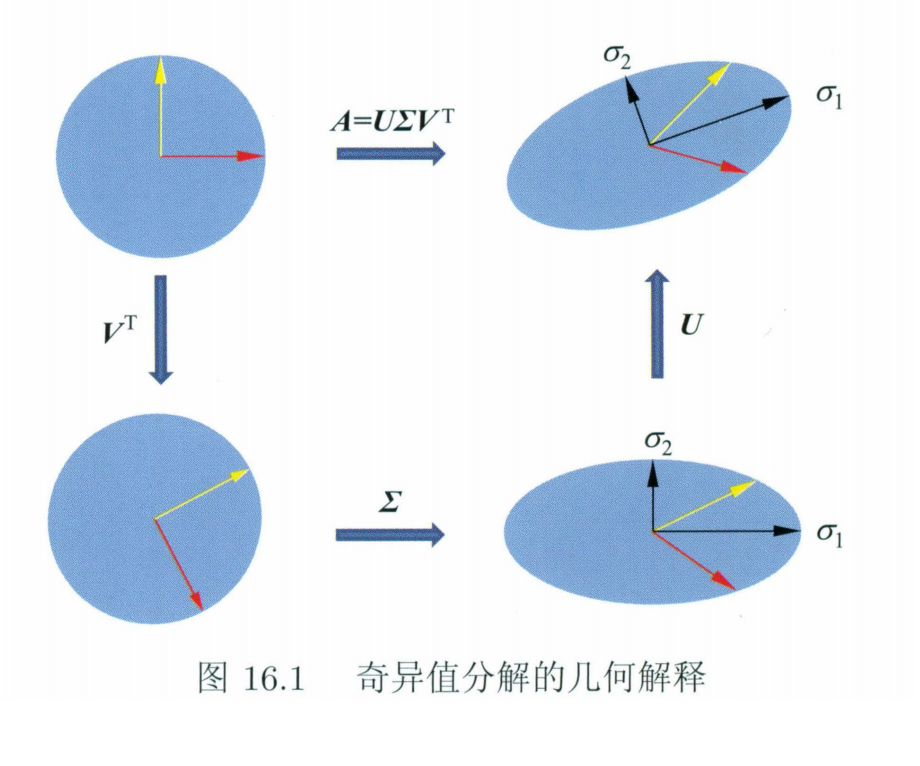
\includegraphics[width=0.6\textwidth]{SVD.png}
            \caption{SVD分解示意图}
        \end{figure}

        由图，$\boldsymbol{V}^T$是$\mathbb{R}^n $上的坐标旋转或者反射变换；$\boldsymbol{\Sigma}$是坐标轴的伸缩变换；$\boldsymbol{U}$是咋$\mathbb{R}^n$上的坐标旋转或者反射变换。
        截断奇异值分解，就是对原始完全的变换做出截断。

        矩阵近似在几何上理解就是近似变换。对原始矩阵$A$直接修改来近似是很难入手的，截断近似提供了一种方法。那么怎么衡量近似的程度呢？
        这个问题一般通过距离或者近似度来衡量。距离往往更加直接，矩阵距离无法直接表示，但是可以
        参考向量的$L2$范数。

        弗罗贝乌斯范数：
        \[\|A\|_F=\left(\sum_{i=1}^{m}\sum_{j=1}^{n}a_{ij}^2\right)^\frac{1}{2}\]

        对于奇异值分解：
        \[\|A\|_F=(\sigma_1^2+\sigma_2^2+\cdots+\sigma_r)^\frac{1}{2}\]

        所以最优近似是解决如下优化问题：假设所有截断矩阵集合为$\mathcal{M}$
        \[\boldsymbol{X}=\arg\min_{\boldsymbol{X}\in\mathcal{M}}\|\boldsymbol{A}-\boldsymbol{X}\|_F^2\]

        这个问题很好解，因为$\boldsymbol{\Sigma}$是由大到小排列的。所以对于特定的k，
        当
        \[\boldsymbol{\Sigma}=\begin{bmatrix}
                \sigma_1&&&&\\
                &\ddots&&&\\
                &&\sigma_k&&\\
                &&&\ddots&\\
                &&&&0\\
        \end{bmatrix}
        =\begin{bmatrix}
            \Sigma_k&0\\
            0&0\\
        \end{bmatrix}
        \]

        \[\|\boldsymbol{A}-\boldsymbol{X}_k\|_F^2=(\sigma_{k+1}^2+\sigma_{k+2}^2+\cdots+\sigma_r^2)\]
        时最优。

    
    \section{近似思路扩展}
        上述解决了最优近似问题。但是在机器学习尤其是数据处理部分的时候，这个近似方法非常多。

        笔者在语义分析的时候使用过奇异值分解。具体就是解决词向量矩阵稀疏的问题，导致这个问题的主要原因是
        数据不够多，直接增大数据集是一种有效的办法。但是增加数据也会出现稀疏或者局部稀疏的问题，这是由于
        数据分布问题导致的，所以压缩数据是数据稠密是必须的。因为这可以提高计算效率也可以减少存储成本。

        可以尝试确定$k$值来截断，但是有一个问题：最优求解是很容易得到的，但是希望压缩的目标不仅仅是贴合原始变换，
        还是需要最优压缩的。这意味着，对于每个$k$还有很多近似矩阵需要查找优化，但是它们的差异其实不算大。

        所以有更跳跃的想法。比如就取矩阵$\boldsymbol{U}$或者$\boldsymbol{V}$或者$\boldsymbol{\Sigma}$或者诸如$\boldsymbol{U}\boldsymbol{\Sigma}$的组合作为
        近似矩阵，这一步可以跳很远。

        还可以有其它的思想，譬如以奇异值为参考，即认为坐标轴变换大的是主要因素，直接提取最主要因素相关的$\boldsymbol{U}$或者相关分解或者组合作为近似矩阵。

        当然，词向量压缩是一个复杂的工作。没有说哪种方法就一定好。

\end{document}